%\documentclass[]{article}
%\usepackage{graphicx}
%\usepackage{subfig}
%\usepackage{amsmath}
%\usepackage{amsfonts}
%\usepackage[margin=1in]{geometry}

%\begin{document}

Now it's time to actually see how well the various algorithms we have discussed performed on our dataset. Throughout this section, we refer to the algorithms with the following names:
\begin{enumerate}
\item svm = svm with linear kernel
\item svm pca = linear kernel svm with 50 dim pca applied first
\item ridge = $L_2$ regularized logistic regression. 
\item lasso = $L_1$ regularized logistic regression.
\item lasso pca = $L_1$ regularized logistic regression w/ 50 dim pca. 
\item naivebayes smooth = naive bayes with `add one' smoothing.
\item naivebayes smooth pca small= naivebayes smooth with 5-dim. pca
\item naivebayes smooth pca = naivebayes smooth with 50-dim. pca
\item naivebayes smooth rand = naivebayes smooth with 50-dim random projection
\end{enumerate}

TODO get new numbers for this. run c3N.m
In table \ref{tab:AccTable}, we list
\begin{center}
\begin{table}
\begin{tabular}{lcc}
\hline
& Mean & STD \\
\hline
svm & .9600 & 2.3406e-16\\
svm pca & 0.9400 & 2.3406e-16\\
ridge & 0.9400 & 2.3406e-16\\
lasso pca & 0.9460 & 0 \\
naivebayes smooth rand & 0.6826 & 0.0226\\
naivebayes smooth pca small & 0.9060 & 0\\
naivebayes smooth pca & 0.7680 & 1.1703e-16\\
lasso & 0.9380 & 0\\
naivebayes smooth & 0.6260 & 1.1703e-16
\end{tabular}
\caption{Performance of various classifiers}
\label{tab:AccTable}
\end{table}
\end{center}


TODO mention something about how looking for regimes didn't quite work because we were subsampling, not making bigger. 
\begin{center}
\begin{figure}[!ht]
\centering
\subfloat[Accuracy]{\includegraphics[width=.7\textwidth]{../images/c3.png}}
\subfloat[Legend]{\includegraphics[width=.3\textwidth]{../images/legend.png}}
\caption{Accuracy vs Size of subsampled training data used}
\label{fig:largecompareAcc}
\end{figure}
\end{center}


Overall, our experiments suggest that sometimes dimensionality reduction is critical when we have little data. To illustrate this phenomenon, in figure \ref{fig:lassoCompare} we vary the size of the training set and compare the accuracy of  $L_1$ regularized logistic regression with and without pca being applied to the data. We find that for extremely small training set sizes, lasso with pca performs substantially better than it does on the raw 17,000 dimensional data. However, as we increase the size of the training set, the performances become comparable. If our dataset had been larger, we would have perhaps identified that the performances cross eventually. 

\begin{center}
\begin{figure}[!ht]
\centering
\includegraphics[width=.7\textwidth]{../images/_lasso_lasso_pca_acc.eps}
\caption{Accuracy vs. Train set size}
\label{fig:lassoCompare}
\end{figure}
\end{center}

	In the background section, we discussed an important result due to Ng and Jordan that logistic regression is asymptotically better than naive Bayes, but naive Bayes approaches its higher asymptotic accuracy more quickly ~\ref{jordan2002discriminative}. In figure \ref{fig:Ngcompare}, we vary the size of the training set and compare logistic regression with pca and logistic naive Bayes with pca. For this dataset, we are not able to identify a regime of small train set sizes where classification performance for naive Bayes is better. Logistic regression is always superior. One defining characteristic of our dataset, which Ng and Jordan don't account for in their arguments, is the very high level of the data, even after 50-dimensional pca projection (50\% sparse). The number of nonzero observations for each observation is quite low, and thus naive Bayes can not estimate its component-wise Gaussian distributions accurately. Logistic regression makes fewer assumptions about the underlying generative process and consequently less vulnerable to sparsity. 
 
\begin{center}
\begin{figure}[!ht]
\centering
\includegraphics[width=.7\textwidth]{../images/_naivebayes_smooth_pca_lasso_pca_acc.eps}
\caption{Which of Ng and Jordan's regimes are we in? Accuracy vs. train set size}
\label{fig:Ngcompare}
\end{figure}
\end{center}


	We found that dimensionality reduction is important to maintain high classification accuracy for some algorithms in the $n << p$ regime. An additional advantage of it is reduction in time and memory requirements for training. In figure \label{fig:timecompare} we plot the time cost of training a naive Bayes model with pca v.s. a naive bayes model without pca. We find that the training time for the raw 17,000 dimensional data (red curve) explodes as we increase the training size. Due to the seemingly linear relationship of time vs. train set size for the red curve for most of the train set sizes, its sudden explosion, and the large error bars on the final measurement, it seems like the laptop the experiment was run on became strained and unreliable. When the memory limits of the computer are approached, it suddenly needs to do lots of work to keep things in place, and as a result, runtimes increase tremendously. 

\begin{center}
\begin{figure}[!ht]
\centering
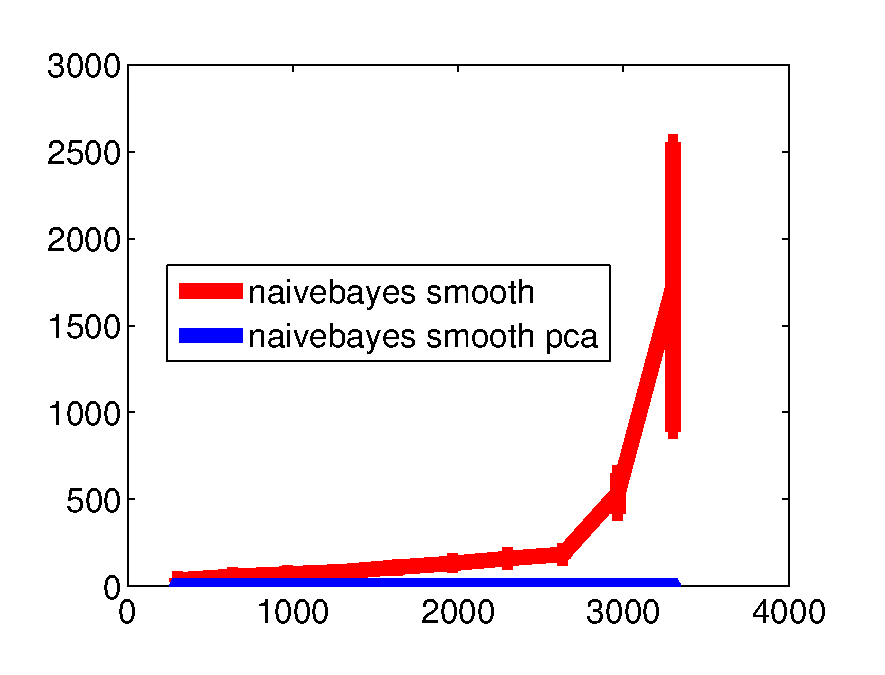
\includegraphics[width=.7\textwidth]{../images/_naivebayes_smooth_naivebayes_smooth_pca_time.eps}
\caption{train time vs. train set size}
\label{fig:timecompare}
\end{figure}
\end{center}


%\end{document} 

